\section{Measurement}
Three measurements were made with the see-through speaker; closed box, bottom-hole open and bottom \SI{0.27}{\litre} bass reflex. One closed box measurement was made with the wooden speaker. The results are shown in \cref{fig:measAll}.

\begin{figure}
	\centering
	\begin{subfigure}{.5\textwidth}
		\centering
		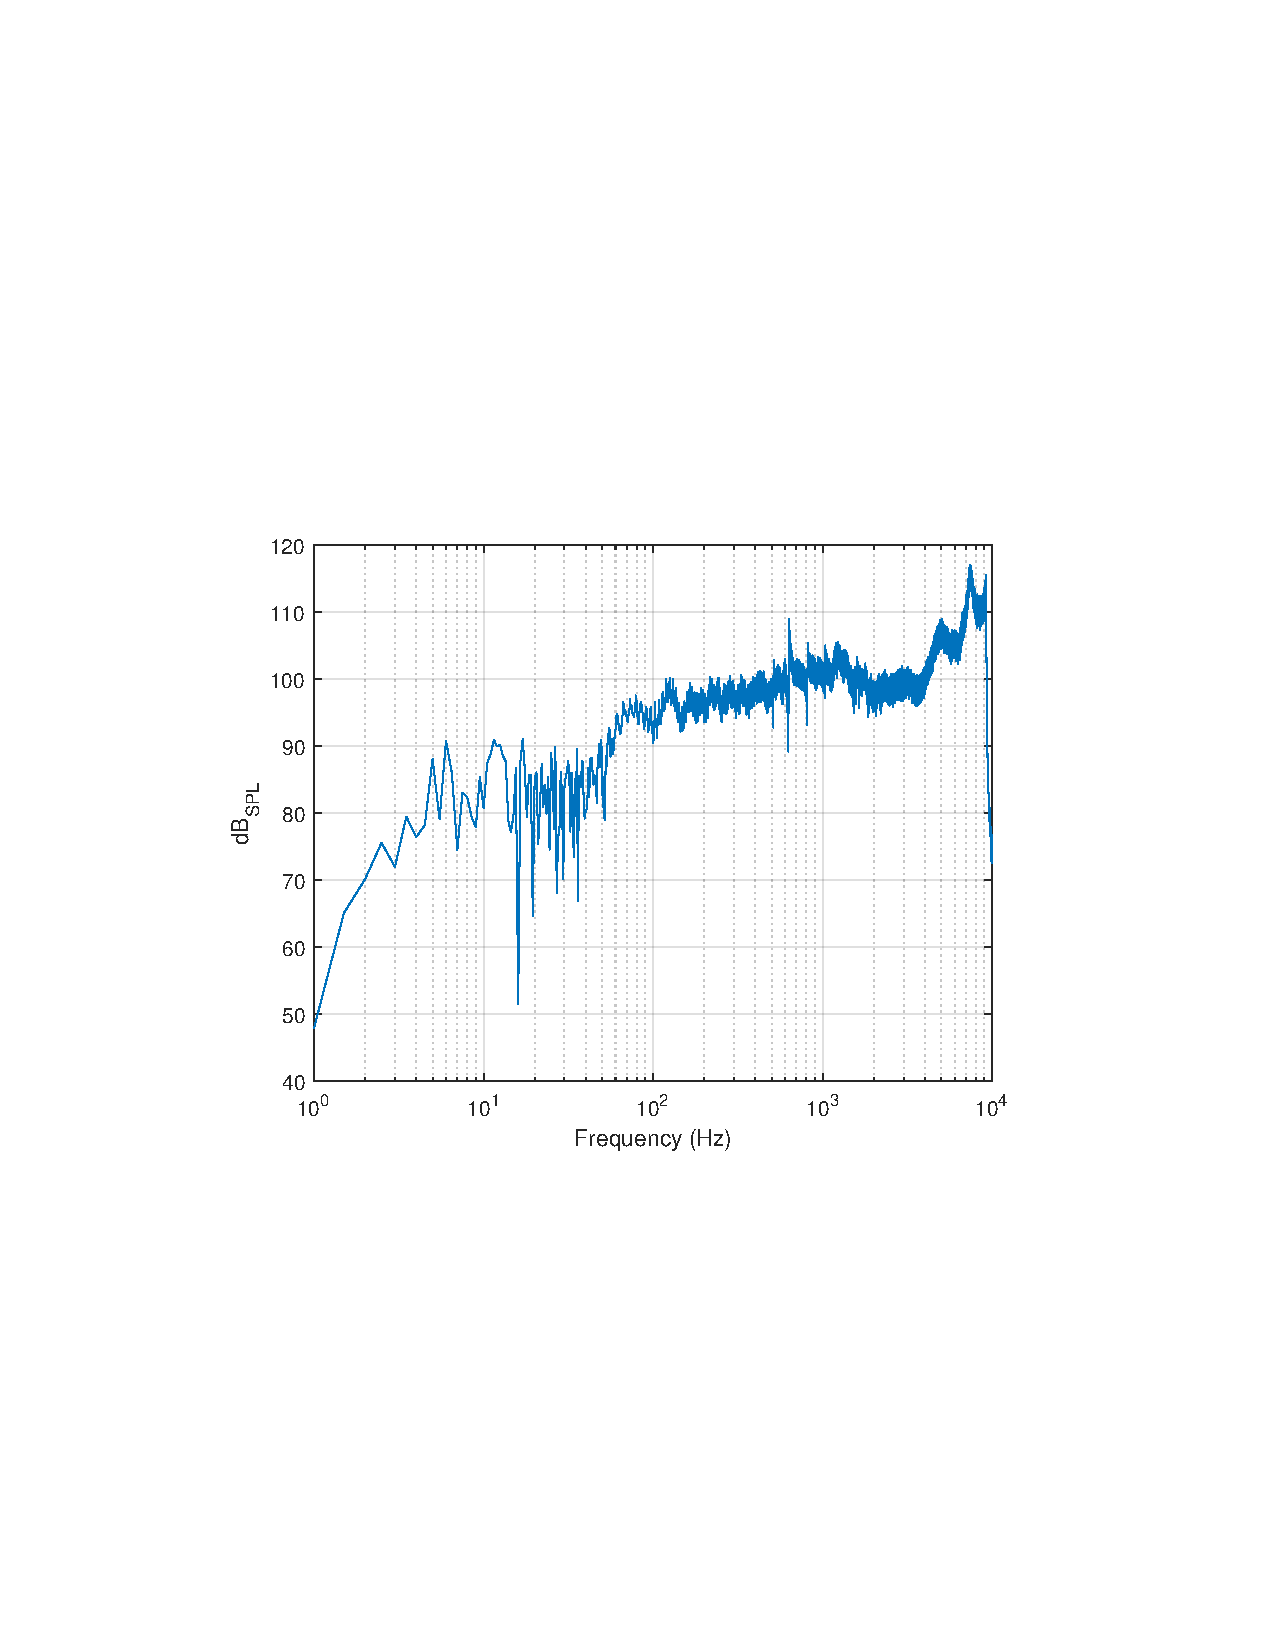
\includegraphics[width=.9\linewidth, clip, trim={3.9cm 8.4cm 4.5cm 9cm}]{gfx/SpeakerMeas/PGclosed.pdf}
		\caption{See-through speaker. All openings sealed.}
		\label{fig:measPGclose}
	\end{subfigure}%
	\begin{subfigure}{.5\textwidth}
		\centering
		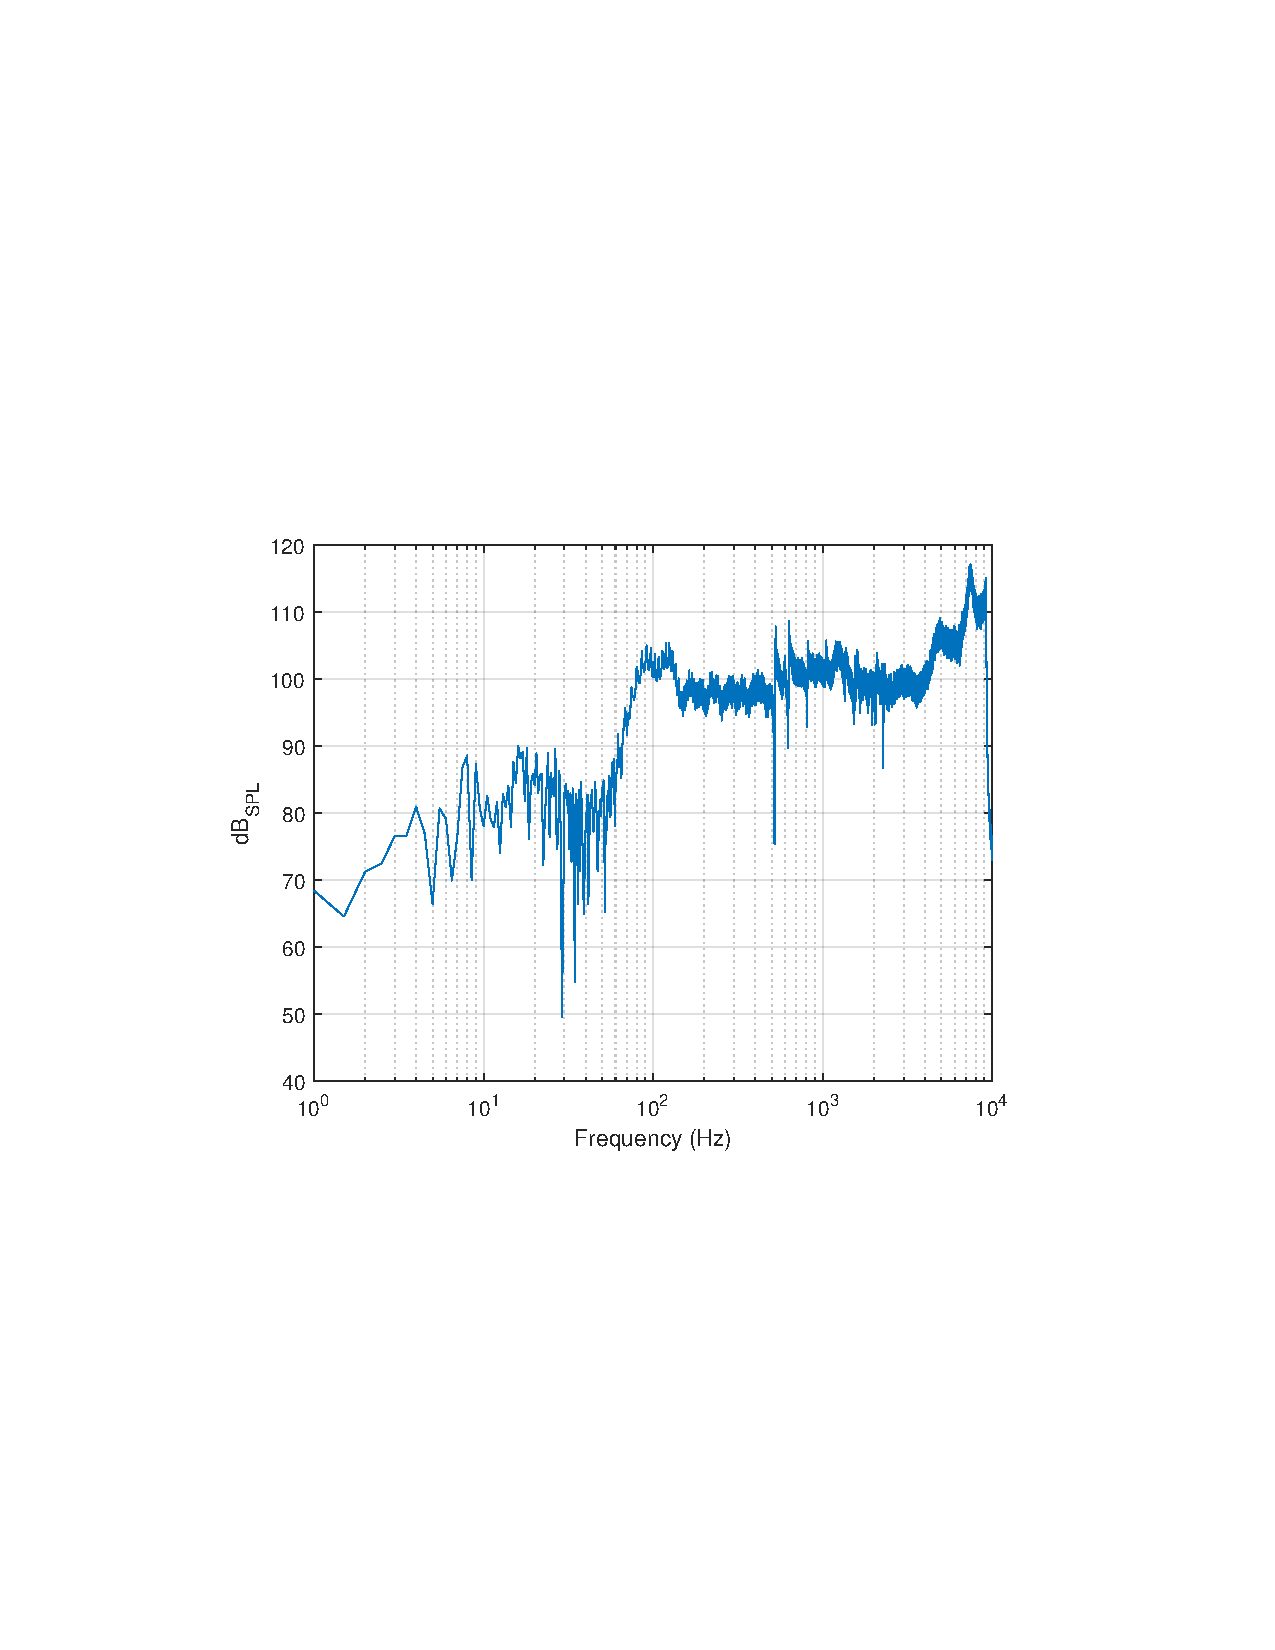
\includegraphics[width=.9\linewidth, clip, trim={3.9cm 8.4cm 4.5cm 9cm}]{gfx/SpeakerMeas/PGopen.pdf}
		\caption{See-through speaker. Bottom opening open.}
		\label{fig:measPGopen}
	\end{subfigure}
	\\
	\begin{subfigure}[t]{.5\textwidth}
		\centering
		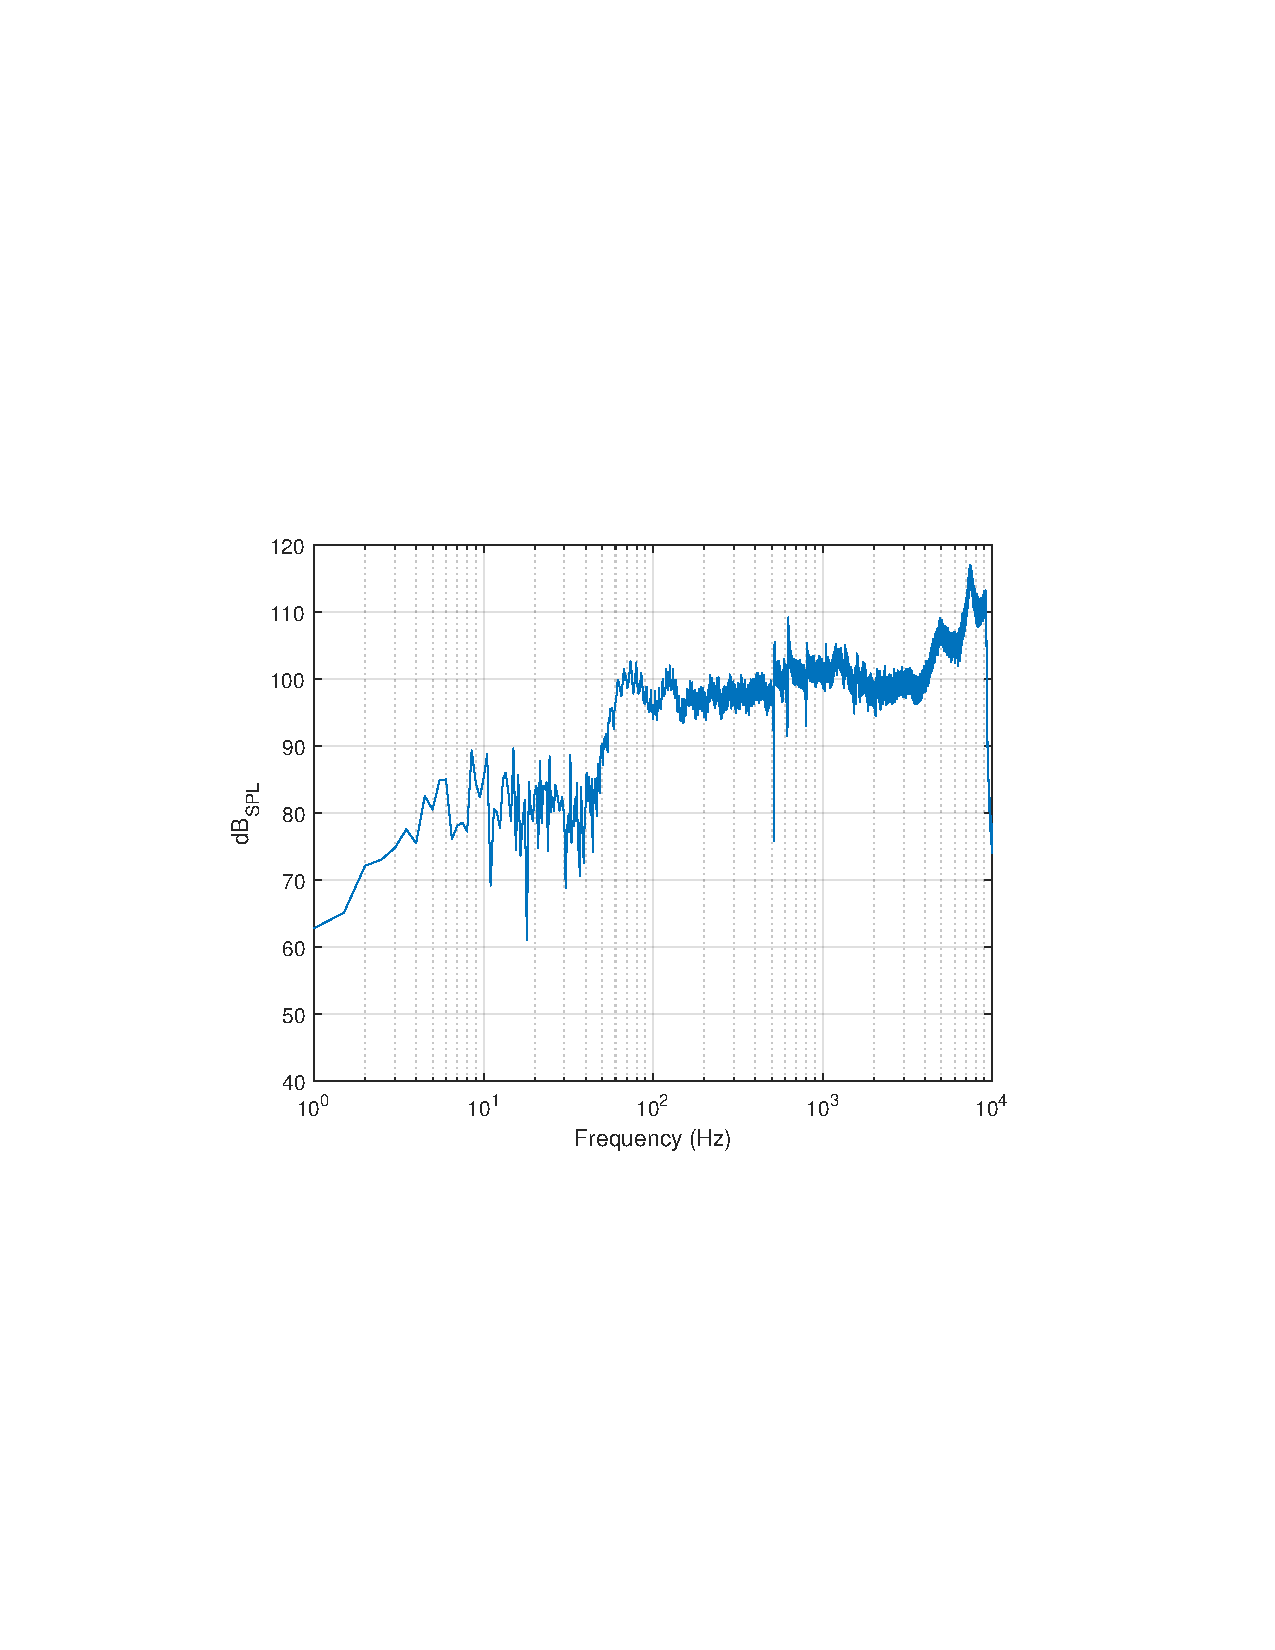
\includegraphics[width=.9\linewidth, clip, trim={3.9cm 8.4cm 4.5cm 9cm}]{gfx/SpeakerMeas/PGBR.pdf}
		\caption{See-through speaker. Bass reflex with length \SI{7}{\centi\metre} and diameter \SI{5}{\centi\metre} inserted at bottom.}
		\label{fig:measPGbass}
	\end{subfigure}%
	\begin{subfigure}[t]{.5\textwidth}
		\centering
		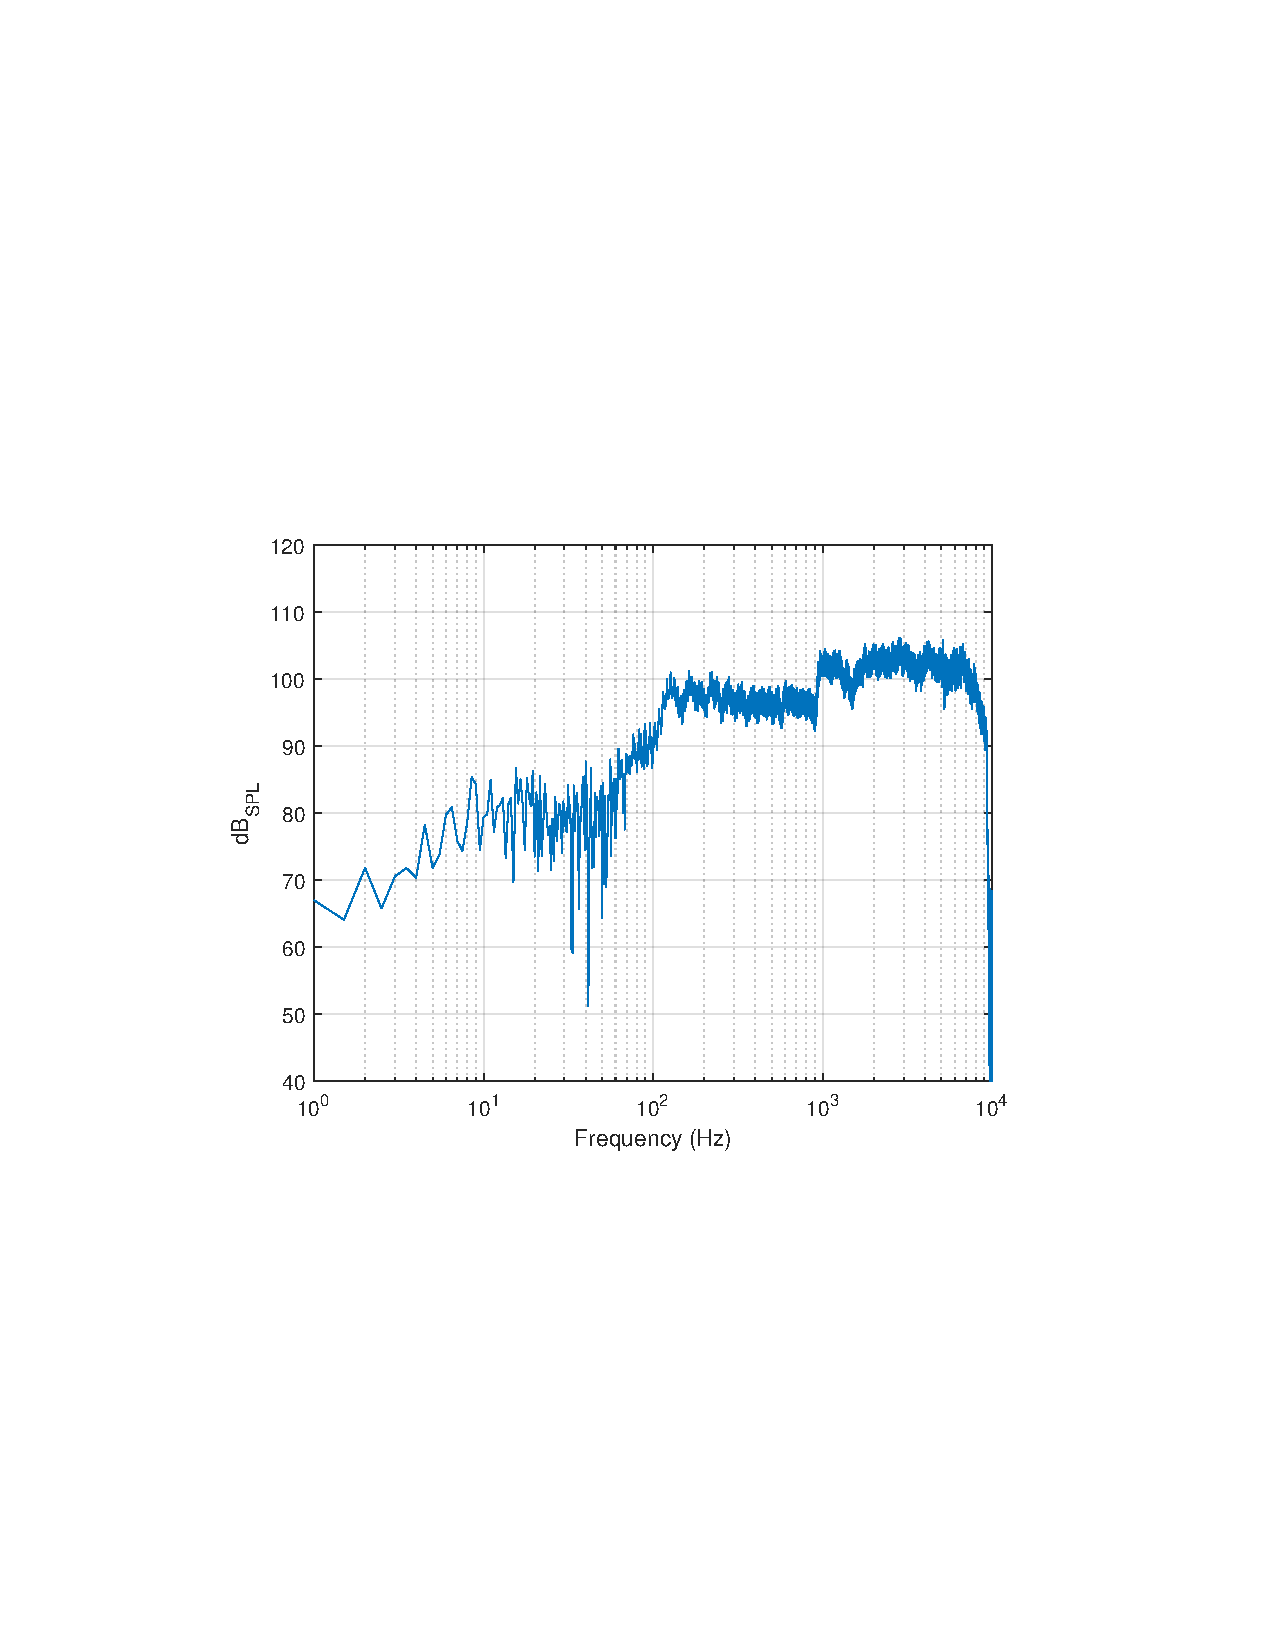
\includegraphics[width=.9\linewidth, clip, trim={3.9cm 8.4cm 4.5cm 9cm}]{gfx/SpeakerMeas/PKclosed.pdf}
		\caption{Wooden speaker measurement.}
		\label{fig:measPK}
	\end{subfigure}
	\caption{Measurements of the speakers.}
	\label{fig:measAll}
\end{figure}

Comparing the closed box approach of both speakers, \cref{fig:closedcompare}, they differ mostly in the regions \SIrange{50}{100}{\hertz} and \SIrange{400}{10000}{\hertz}.
This is most likely due to different Thiele/Small parameters.
It should be noted that the closed box measurements does not exhibit a spike at the resonance frequency, which indicates that the cabinets where not hermetically sealed.

\begin{figure}
	\centering
	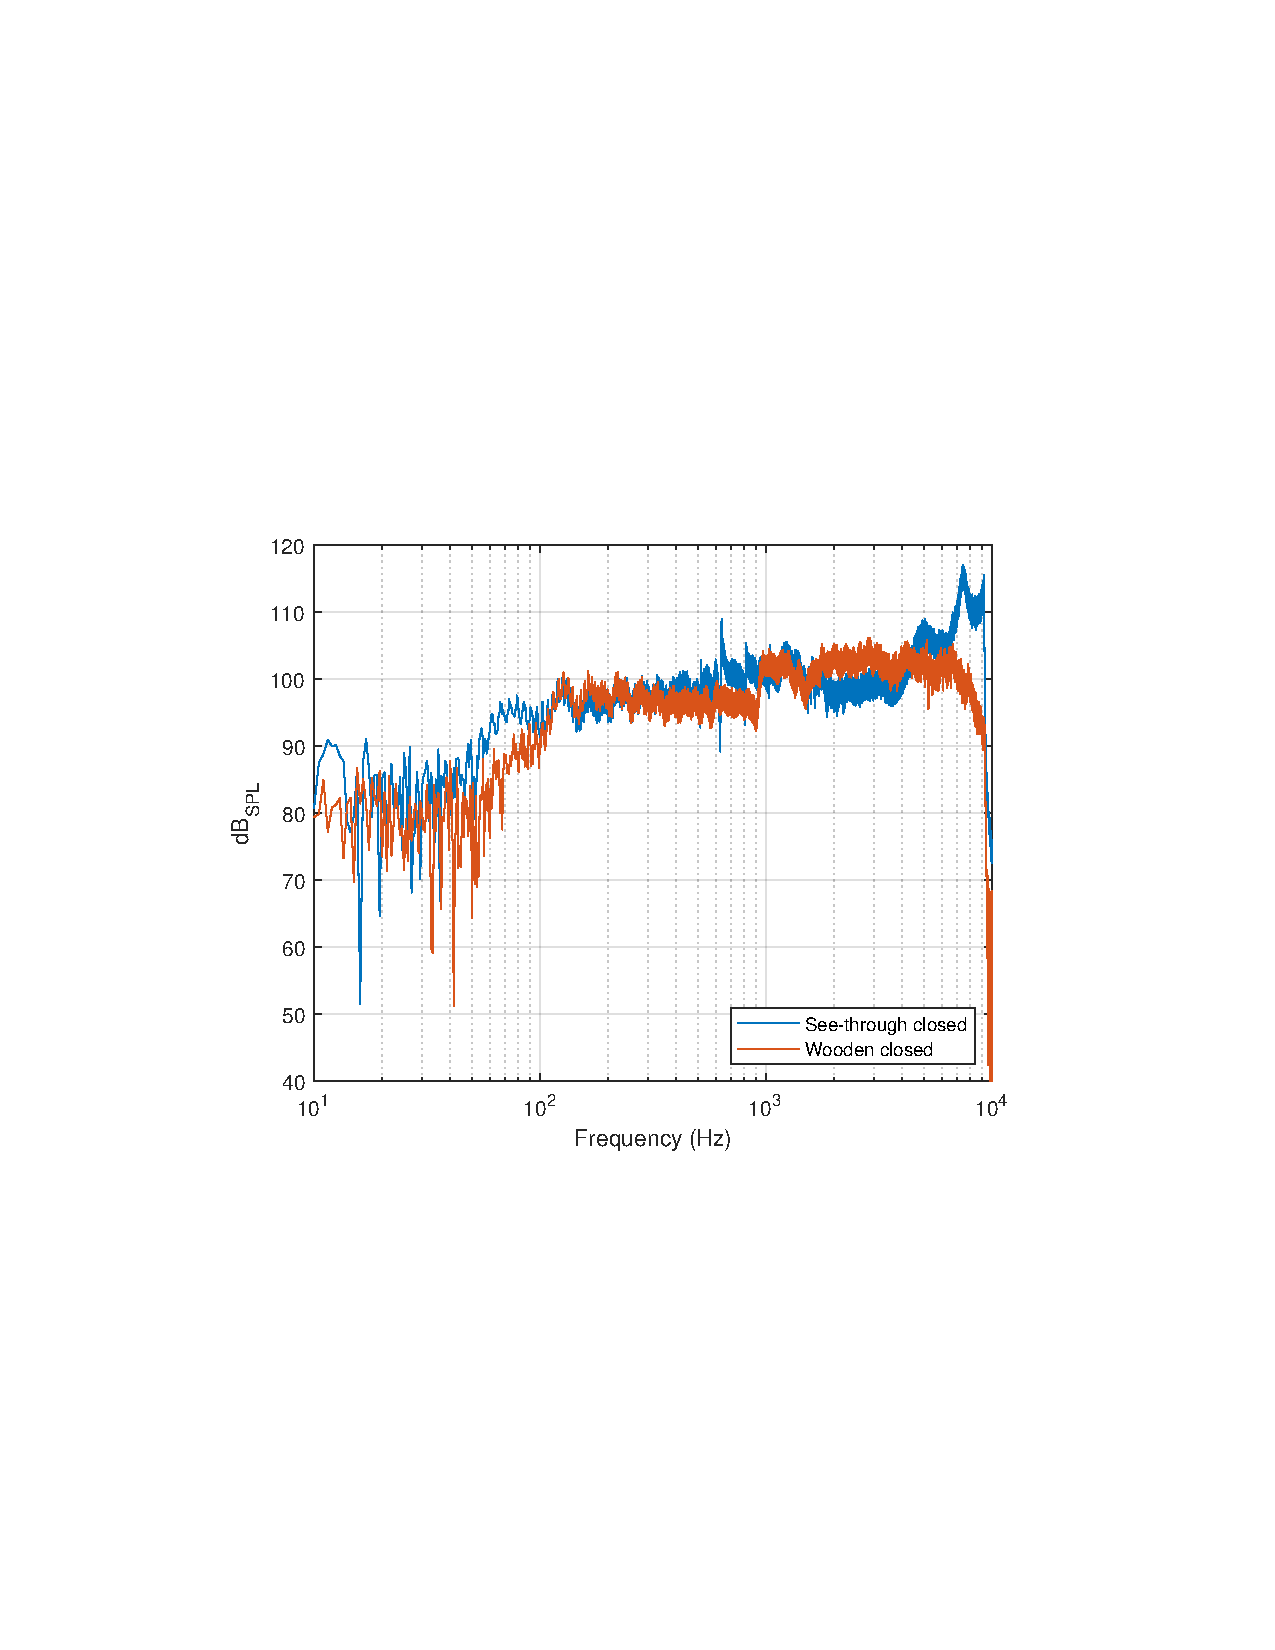
\includegraphics[width=0.7\linewidth, clip, trim={3.9cm 8.4cm 4.5cm 9cm}]{gfx/SpeakerMeas/ClosedCompare.pdf}
	\caption{Comparison of see-through closed and wooden.}
	\label{fig:closedcompare}
\end{figure}

When comparing the see-through speaker setups, \cref{fig:PGcompareAll}, the responses are very similar, except for in the range \SIrange{50}{150}{\hertz}, \cref{fig:PGcompareZoom}.
This is the range at which the response goes from a slope of \SI{12}{\decibel}/octave for the closed setup, and \SI{24}{\decibel}/octave for the open and bass reflex setups, to a more linear frequency response.
Here the gain from using a bass reflex gives approximately \SIrange{3}{5}{\decibel} in the range \SIrange{60}{90}{\hertz}.

\begin{figure}
	\centering
	\begin{subfigure}{.5\textwidth}
		\centering
		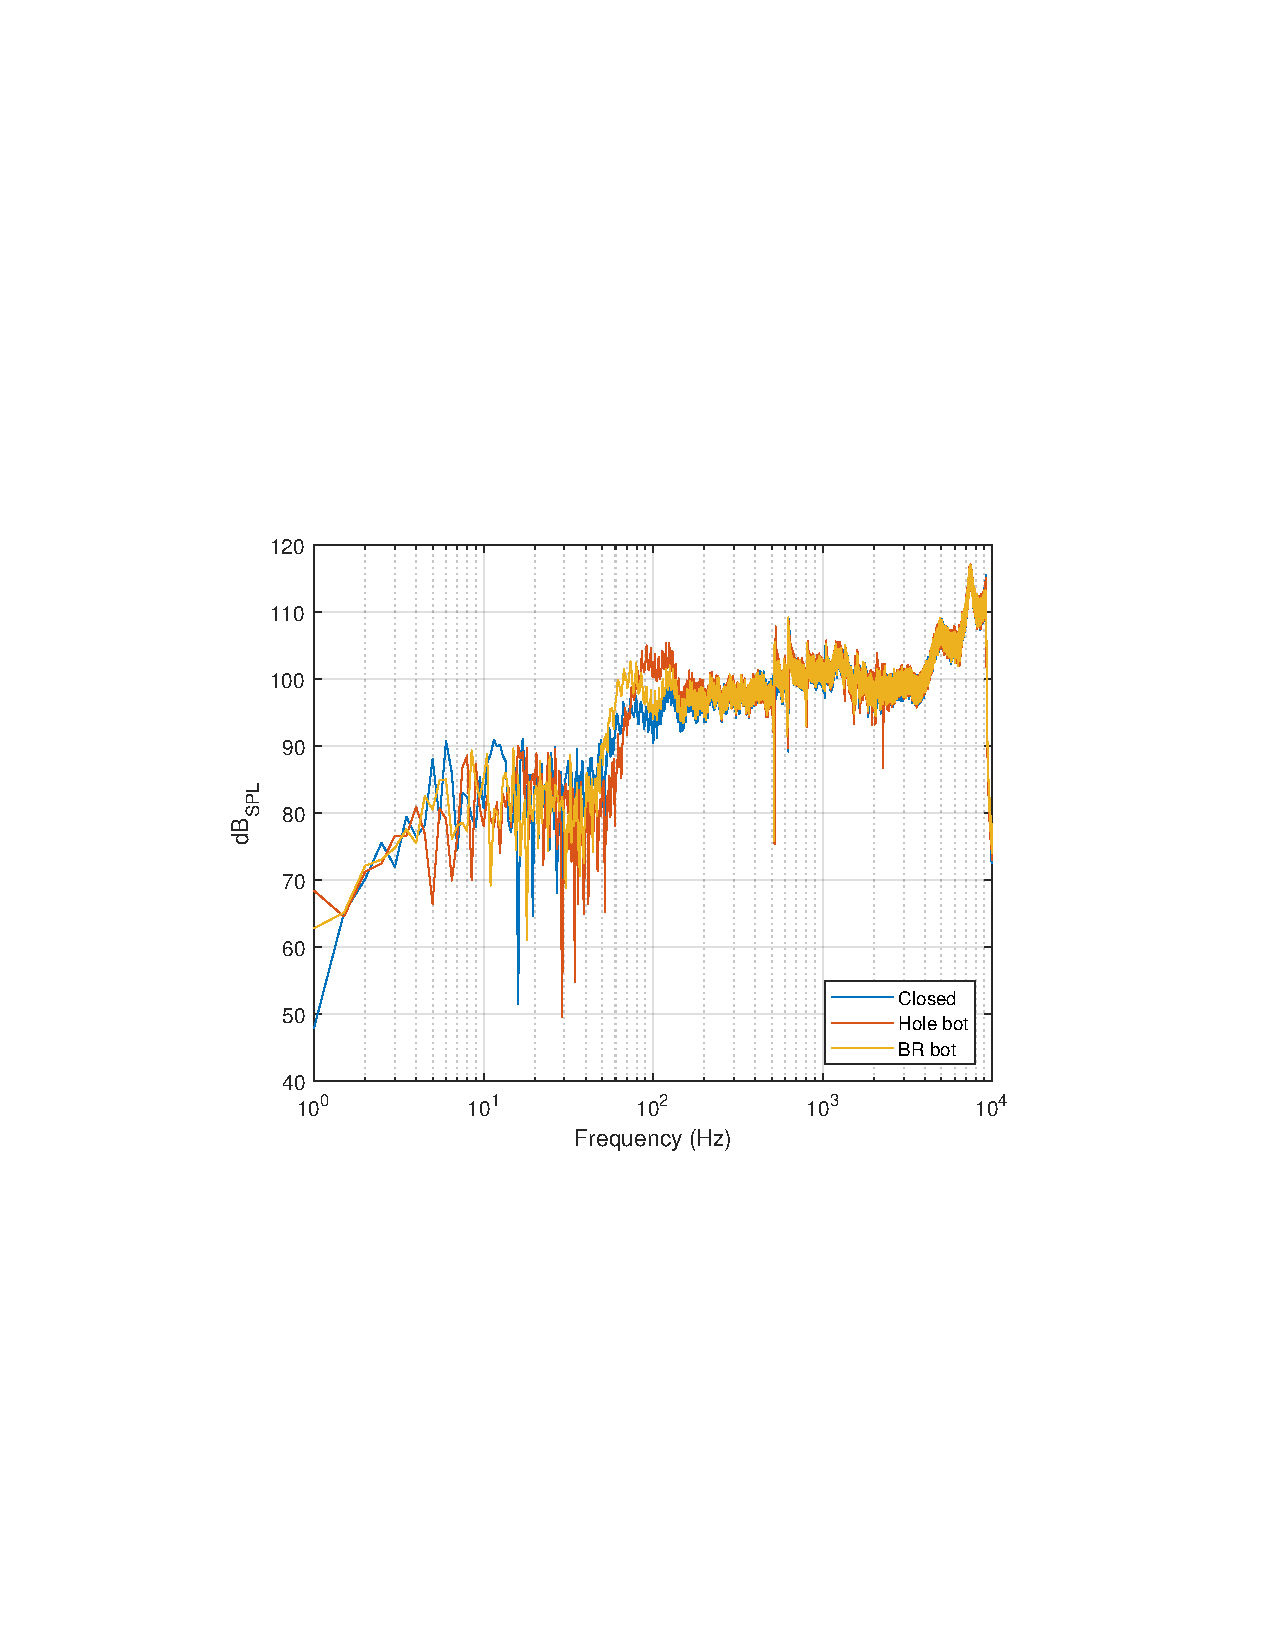
\includegraphics[width=.9\linewidth, clip, trim={3.9cm 8.4cm 4.5cm 9cm}]{gfx/SpeakerMeas/PGcompare.pdf}
		\caption{See-through speaker.}
		\label{fig:PGcompareAll}
	\end{subfigure}%
	\begin{subfigure}{.5\textwidth}
		\centering
		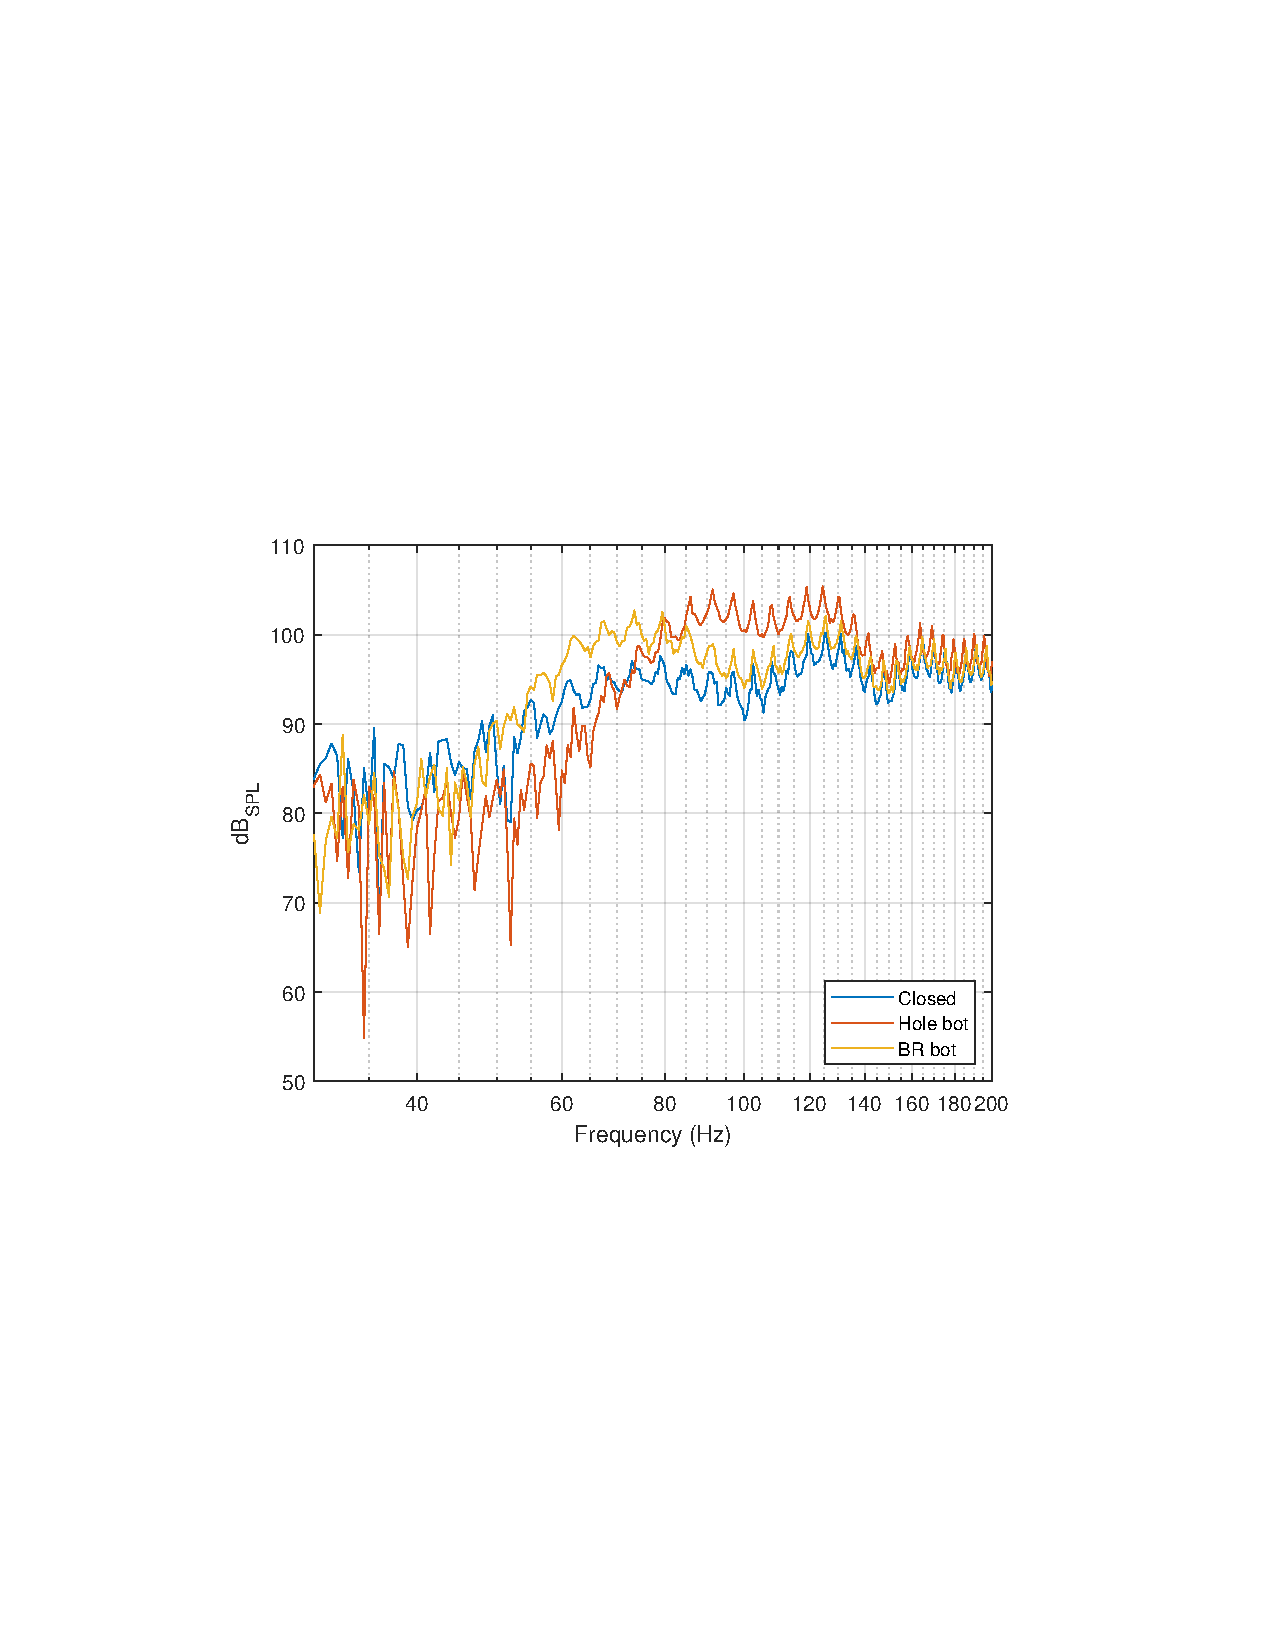
\includegraphics[width=.9\linewidth, clip, trim={3.9cm 8.4cm 4.5cm 9cm}]{gfx/SpeakerMeas/PGcompareZoom.pdf}
		\caption{Zoom of \cref{fig:PGcompareAll}.}
		\label{fig:PGcompareZoom}
	\end{subfigure}
	\caption{Comparison of the different setups of the see-through speaker.}
	\label{fig:PGcompare}
\end{figure}

\FloatBarrier